\makeatletter
\def\input@path{{../}}
\makeatother
\documentclass[../Thesis.tex]{subfiles}
\begin{document}
\chapter{Multiwavelet Basis}\label{chap:MW_basis}
As stated in the previous chapter \ref{chap:Quantum_chemistry}, the main goal of computational chemistry is
to approximate systems in order to calculate their energy through the \ac{SE}. %cite please
These systems are completely described by wave functions \cite{Cohen:1973}.


In order to construct a solution (wave function) to the \ac{SE} of a given
system one uses sets of functions with differing properties. These
sets of functions construct a basis for the space on which the wave functions
are projected into. These sets are thus called basis sets \cite{Cramer:2004}
and they are essential to solving many-body systems. In this text we will be
focusing in the \ac{MW} basis from \ac{MRA} methods.

\section{Different types of basis sets}
We have mentioned constructing solutions of systems using basis sets represented as
\ac{LCAO}, sums of basis functions multiplied with projection coefficients.
In this section we discuss some basis sets used to solve quantum chemical systems.

\subsection{Atom centered basis sets}
Some of the first basis sets to be developed were based on the assumption of
centering the functions on the atom nucleus. These basis sets are called \ac{STO}
and \ac{GTO}. The basis functions (orbitals) follow from the separation of variables
used in solving for one-electron atoms
\begin{equation}
  \Psi(\rvec) = R(r)Y_{lm}(\theta, \phi),
\end{equation}
where $R$ is the radial part of the wave function and $Y$ is the angular part of
the wave function.

\subsubsection{Slater-type orbitals}
These basis functions are constructed from the observation that the wave function
should decay exponentially to zero when the distance from the nucleus extends
to infinity. They are typically of the form \cite{Jensen:2017, ESQCB1P1}
\begin{equation}
  \chi^{STO}(\rvec) = P(r)e^{-\zeta r}Y_{lm}(\theta, \phi),
\end{equation}
where $P$ is a polynomial representing the radial decay and $\zeta$ represents the
how diffuse the function is. These functions are characterized for them having a cusp
at the nucleus, which follows from the treatment of the nucleus as a point charge.
This cusp makes computing integrals and derivatives a complex problem.

\subsubsection{Gaussian-type orbitals}
\ac{GTO} are based on the same reasoning behind \ac{STO}, but instead of letting
the exponential decay be to the rate of  $r$ we let it be to the rate of $r^2$,
that is, we work with Gaussian functions \cite{ESQCB1P1}.
They have the following
forms, both polar coordinates
\begin{equation}
  \chi^{GTO}(\rvec) = P(r)e^{-\alpha r^2}Y_{lm}(\theta, \phi),
\end{equation}
and Cartesian coordinates
\begin{equation}
\chi^{GTO}(\rvec) = (x - A_x)^k(y - A_y)^l(z - A_z)^me^{-\alpha\abs{\rvec - \vec{A}}^2},
\end{equation}
where the vector $\vec{A}$ and its components represent the center of the atom.
In this basis we remove the problem the \acp{STO} had of trying to evaluate the
cusp of the function. The lack of a cusp also allows to treat the nucleus as
more than a point charge. Another advantage is the fact that the functions are no
longer constrained to a spherical coordinate system and can be evaluated on Cartesian
coordinates. They are also separable in the Cartesian coordinate system as a product of
one variable Gaussians.

On the other hand, the \ac{GTO} decay too fast in comparison to the \ac{STO} and
do not describe the nucleus cusp correctly either, meaning that we have to make
more considerations to the exponents and possibly have more
functions per atom in order to find better solutions.

\subsubsection{Contracted Gaussian-type orbitals}
In order to diminish the problem of the cusp in \ac{STO} one tries to represent the
\ac{STO} as linear combinations of \acp{GTO}. This way the decay is properly modeled and the
cusp is no longer a difficult problem to solve. This has the obvious weakness of needing
to compute more basis functions for a single orbital, which increases the cost of running
the calculations \cite{Cramer:2004}. In order to remove this we define the \acp{GTO}
as being represented by another linear combination of \acp{GTO}, but the coefficients for
this one are known and static. This way we can have a better representation of \acp{STO}
with \acp{GTO} \cite{Jensen:2017}.

\subsection{Periodic basis sets}
Periodic basis sets are a type of basis sets that are not centered on an atom.
These basis sets are best at describing, as the name implies, systems with periodic
boundary conditions. Two examples are metals and ion crystals.

\subsubsection{Plane wave basis functions}
In metals, one can think of the valence electrons as free electrons with
periodic boundary conditions. The wave functions of these type of systems are
described by either complex exponentials or cosine and sine functions \cite{Jensen:2017}.

On infinite systems the molecular orbitals, due to the space between different energy levels
vanishing, can be described by a basis of plane waves. The definition in three dimensions
is then a complex exponential.

To finish this section on basis sets we can comment on the applicability of these
basis sets. Atom based basis sets are best at describing the electrons nearest the
nucleus. \acp{STO} are more accurate in the decay, but the cusp at the nucleus is
harder to differentiate, therefore, \ac{GTO} basis sets are used to simplify the
near nucleus differentiation. \acp{GTO} do not decay in the correct manner so one
might want to use contracted \acp{GTO}.

Plane wave functions excel at describing slowly varying delocalized electron densities.
An example is the valence and conduction bands in metal. They are not that good at
describing internal electrons, where the oscillation frequency near the nuclei need to increase a lot
in order to properly approximate the orbital \cite{Jensen:2017}.

\section{Multiresolution analysis}
\subsection{Definition}
Consider that we have a function $\varphi \in L^2(\Real)$ where its translations
and dilations are described as \cite{Schneider:2007}
\begin{equation}
  \varphi^j_k(x) = 2^{\frac{j}{2}}\varphi(2^jx - k),\  j,k \in \mathbb{Z},
\end{equation}
and the function $\varphi(x)$ satisfies the two-scale difference relations \cite{Beylkin:MRA, Schneider:2007, Sorland}
\begin{align}
  \begin{split}
    \varphi(x) &= \varphi(2x) + \varphi(2x - 1),\\
    \varphi^j_k(x) &= \varphi^{j+1}_{2k}(2^{j+1}x - 2k) + \varphi^{j+1}_{2k+1}(2^{j+1}x - 2k - 1),
  \end{split}
\end{align}
where $j$ is the scale of the function and $k$ is the translation of the function
\cite{Sorland}. A normalization constant is included in the definition of $\varphi$.
A space $V^n$ is spanned by translations of $\varphi_{nk}$. This space forms a
hierarchical chain of linear
subspaces \cite{Beylkin:MRA}
\begin{equation}
  V^0 \subset V^1 \subset ... \subset V^j \subset ... \subset L^2(\Real)\label{eq:seqsubspace},
\end{equation}
where $V^0$ is spanned only by $\varphi_{0,0}(x)=\varphi(x)$ \cite{Sorland}.

If relation \ref{eq:seqsubspace} and the following refinement equation holds for $\varphi_{j,k}(x)$
one can call the subspaces $V^n$ or the functions $\varphi_{j,k}(x)$ build a \ac{MRA} of $L_2(\Real)$.
\begin{equation}
\varphi^j_k(x) = \sum_{k\in\mathbb{Z}} h^{j+1}_k\varphi^{j+1}_k(x),
\end{equation}
where $h$ is a coefficient characteristic to the transformation between scales.

\subsection{The Haar wavelet}
From now we will work with the Haar basis for simplicity \cite{Beylkin:MRA}.
Let us define the Haar function \cite{Schneider:2007} as
\begin{equation}
  \varphi^0_0 = \varphi(x) =
  \begin{cases}
  1 & \text{for} \ x\in [0,1)\\
  0 & \text{elsewhere}
\end{cases}.
\end{equation}
Let us now define a second set of subspaces $W^n$. These are the orthogonal complements of $V^n$ \cite{Alpert1993}, also called difference subspaces,
defined as \cite{Beylkin:MRA, Sorland, Alpert1993}
\begin{equation}
  W^n \oplus V^n = V^{n + 1}. \label{eq:diffsubspace}
\end{equation}
The subspaces $W^n$ are then spanned by a set of functions defined by the translations and
dilations of $\psi(x)$
\begin{equation}
  \psi_k^j(x) = 2^{\frac{j}{2}}\psi(2^jx - k),\  j,k \in \mathbb{Z} \label{eq:haarwavelet},
\end{equation}
where $\psi(x)$ is called the Haar wavelet \cite{Schneider:2007} and is defined as
\begin{equation}
  \psi^0_0 = \psi(x) =
  \begin{cases}
  1 & \text{for} \ x\in [0,\frac{1}{2})\\
  -1 & \text{for}\ x\in [\frac{1}{2}, 1),\\
  0 & \text{elsewhere}
\end{cases}
\end{equation}
and $\varphi$ is related to $\psi$ by the following two-scale difference relation \cite{Beylkin:MRA, Schneider:2007, Sorland}:
\begin{align}
  \begin{split}\label{eq:2scalewavelet}
    \psi(x) &= \varphi(2x) - \varphi(2x - 1),\\
    \psi^j_k(x) &= \psi^{j+1}_{2k}(2^{j+1}x - 2k) + \psi^{j+1}_{2k+1}(2^{j+1}x - 2k - 1).
  \end{split}
\end{align}
The functions $\varphi^j_k$ and $\psi^j_k$ are orthonormal
and dense in $L^2(\Real)$ \cite{Beylkin:MRA, Sorland, SRJensen:2014}.

The definition on Equation \ref{eq:diffsubspace} can be applied recursively in order to
get any space $V^n$ as long as one knows the first subspace $V^0$ and one has a method for constructing the
subspace $W^m$ from $V^0$ and $W^{m-1}$
\begin{equation}
    V^0 \oplus W^0 \oplus W^1 \oplus ... \oplus W^{n-1}  = V^n. \label{eq:recursivespace}
\end{equation}

Projecting a function $f(x)$ onto this basis would be then a weighted linear combination
of the Haar functions, but taking into account the definition on Equation \ref{eq:recursivespace} one arrives
at \cite{Sorland}
\begin{equation}\label{eq:projectftohaar}
  f(x)\approx \sum^{2^j -1}_k s^j_k\varphi^j_k = s^0_0\varphi^0_0 + \sum^{N - 1}_j\sum^{2^j -1}_k d^j_k\psi^j_k,
\end{equation}
where $d$ are the difference coefficients and $s$ are the scaled averages of dyadic intervals of the function $f(x)$.

The scaling coefficients $s^j_k$ are computed by the projection $\braket{\varphi^j_k(x)|f(x)}$.
Likewise, the difference coefficients $d^j_k(x)$ are computed by the projection \newline$\braket{\psi^j_k(x)|f(x)}$.
Because of the way the Haar function is defined, we can define  the scaling coefficients as
scaled averages of $f(x)$ at intervals $2^{-j}$ \cite{Sorland, Beylkin:MRA}
\begin{equation}
  s^j_k = \int_{\Real}\varphi^j_k(x)f(x)\text{d}x = \int^{2^{-j}(k + 1)}_{2^{-j}k} f(x) \text{d}x\label{eq:scalecoeff1}.
\end{equation}
The subsequent scaling coefficients can be obtained as
\begin{align}
  \begin{split}\label{eq:scalecoeffint}
    s^{j}_k &= \int_{\Real}\varphi^{j-1}_k(x)\text{d}x\\
            &= 2^{\frac{j}{2}}\int_{\Real}\varphi(2^{j}x - k)f(x)\text{d}x\\
            &= 2^{\frac{j}{2}}\int_{2^{-j}(k-1)}^{2^{-j}k}f(x)\text{d}x.\\
  \end{split}
\end{align}
We can then obtain the difference coefficients by using Equations \ref{eq:scalecoeff1}, \ref{eq:haarwavelet} and \ref{eq:2scalewavelet}:
\begin{align}
  \begin{split}\label{eq:diffcoeffint}
    d^{j - 1}_k &= \int_{\Real}\psi^{j-1}_k(x)f(x)\text{d}x\\
                &= 2^{\frac{j - 1}{2}}\int_{\Real}\psi(2^{j-1}x - k)f(x)\text{d}x\\
                &= 2^{\frac{j - 1}{2}}\left(\int_{\Real}\varphi(2^jx - 2k)f(x)\text{d}x  - \int_{\Real}\varphi(2^jx - 2k - 1)f(x)\text{d}x\right)\\
                &= 2^{\frac{j - 1}{2}}\left( \int^{2^{-j}(2k+1)}_{2^{-j}2k}f(x)\text{d}x - \int^{2^{-j}(2k+2)}_{2^{-j}(2k + 1)}f(x)\text{d}x \right)\\
                &= \frac{1}{\sqrt{2}}\left(s^{j}_{2k} - s^{j}_{2k+1} \right).
  \end{split}
\end{align}

The result of Equations \ref{eq:diffcoeffint} and \ref{eq:scalecoeffint} show us
that we can represent the projection of coefficients onto a coarser scale as an
orthogonal matrix \cite{Sorland, Beylkin:MRA}:
\begin{equation}
  \begin{pmatrix}
    d^{j}_k \\
    s^{j}_k
  \end{pmatrix} =
  \begin{pmatrix}
    \frac{1}{\sqrt{2}} & -\frac{1}{\sqrt{2}} \\
    \frac{1}{\sqrt{2}} & \frac{1}{\sqrt{2}}
  \end{pmatrix}
  \begin{pmatrix}
    s^{j+1}_{2k} \\
    s^{j+1}_{2k+1}
  \end{pmatrix}.
\end{equation}
Projecting the coefficients into a more refined scale is just a transpose of the
above matrix:
\begin{equation}
  \begin{pmatrix}
    s^{j+1}_{2k} \\
    s^{j+1}_{2k+1}
  \end{pmatrix} =
  \begin{pmatrix}
    \frac{1}{\sqrt{2}} & \frac{1}{\sqrt{2}} \\
    -\frac{1}{\sqrt{2}} & \frac{1}{\sqrt{2}}
  \end{pmatrix}
  \begin{pmatrix}
    d^{j}_k \\
    s^{j}_k
  \end{pmatrix}.
\end{equation}

\subsection{Projecting a Gaussian function example}
As an example, let us approximate the function
$f(x) = \frac{10}{\sqrt{\pi}}e^{-100(x - 0.5)^2}$ in $L^2(\Real)$
with Haar basis up to scale $5$ using \ref{eq:projectftohaar}. This gives us the
plots in the following Figure \ref{fig:Hargaussproject}.

\begin{figure}[h!]
  \centering
  \begin{subfigure}[b]{0.49\linewidth}
    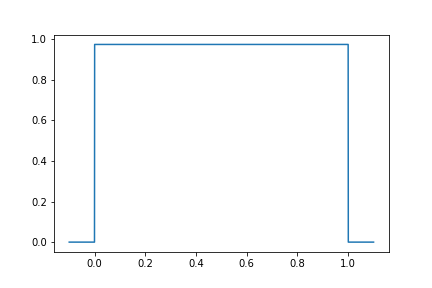
\includegraphics[width=\linewidth]{img/scale1.png}
    \caption{Haar basis projection to the 1st scale}
  \end{subfigure}
  \begin{subfigure}[b]{0.49\linewidth}
    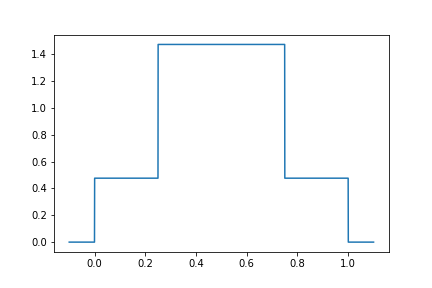
\includegraphics[width=\linewidth]{img/scale2.png}
    \caption{Haar basis projection to the 2nd scale}
  \end{subfigure}
  \begin{subfigure}[b]{0.49\linewidth}
    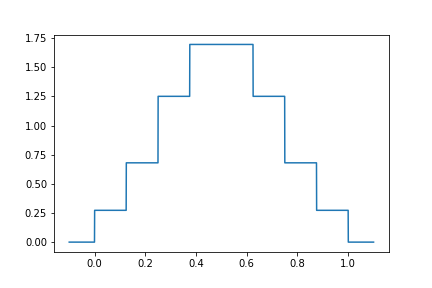
\includegraphics[width=\linewidth]{img/scale3.png}
    \caption{Haar basis projection to the 3rd scale}
  \end{subfigure}
  \begin{subfigure}[b]{0.49\linewidth}
    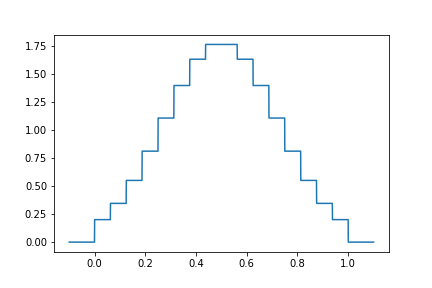
\includegraphics[width=\linewidth]{img/scale4.png}
    \caption{Haar basis projection to the 4th scale}
  \end{subfigure}
  \begin{subfigure}[b]{0.49\linewidth}
    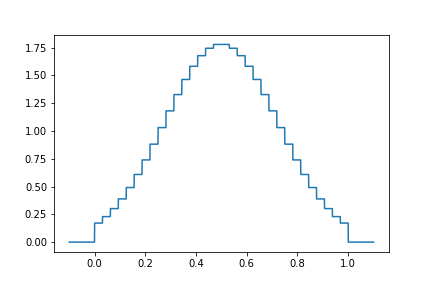
\includegraphics[width=\linewidth]{img/scale5.png}
    \caption{Haar basis projection to the 5th scale}
  \end{subfigure}
  \begin{subfigure}[b]{0.49\linewidth}
    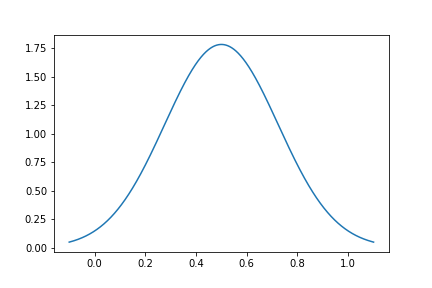
\includegraphics[width=\linewidth]{img/gaussian.png}
    \caption{Analytical plot of $f(x)$}
  \end{subfigure}
  \caption[Projecting a Gaussian function with Haar basis]{Projecting Gaussian function $f(x) = \frac{10}{\sqrt{\pi}}e^{-100(x - 0.5)^2}$ with
  Haar basis up to scale 5 on interval $(0, 1)$}
  \label{fig:Hargaussproject}
\end{figure}


\section{Multiwavelet \ac{MRA}}
\subsection{Constructing the basis functions in one dimension}
Following the same basics as in the Haar basis from the previous section we can
define a hierarchical set of multiresolution spaces $V^j_l$ where \cite{Frediani:2013}
\begin{align}
  \begin{split}
    V^j_l \defeq \{&f: \text{all polynomials of degree} \leqslant
    l\  \\
    &\text{on}\  (2^{-j}k,2^{-j}(k+1))\ \text{for}\ 0\leqslant k < 2^{n},\\
    &f\  \text{vanishes elsewhere}\}
  \end{split}
\end{align}
and
\begin{equation}
  V^0_l \subset V^1_l \subset ... \subset V_l^j \subset ... \subset L^2(\Real).
\end{equation}

We again define subspaces $W^^l$ as the orthogonal complements of $V^l_j$
\cite{Alpert1993} defined as
\begin{equation}
  V_l^j \oplus W^j_l = V_l^{j+1},
\end{equation}
 with orthogonal basis functions  $\psi^j_{lk}$ which are translations and dilations of functions $\psi_i$
 \begin{equation}
   \psi^j_{ik}(x) = 2^\frac{j}{2}\psi_i(2^jx-k), \ i=1, ...,l;\ k \in \mathbb{Z}.\label{eq:mwbasisfuncs}
 \end{equation}
 The functions $\psi_1, ...,\psi_l$ are piece-wise polynomial, orthogonal to lower order polynomials and
 vanish outside $[0,1]$ and their subscripts denote the polynomial order \cite{Alpert1993}
\begin{align}
  \int_0^1\psi_i(x)x^m \text{d}x = 0,\ m = 0, 1, ..., l-1.
\end{align}

 The basis functions $\phi_i(x)$ of the subspace $V_l^0$ can be defined using the following two-scale
difference equations \cite{Beylkin1999AdaptiveSO}, which are analogous to the
two-scale difference equations in \ref{eq:2scalewavelet}
\begin{align}
  \psi_i(x) &= \sqrt{2}\sum^{l-1}_{j=0}\left(\bar{H}^{(0)}_{ij}\psi_j(2x) + \bar{H}^{(1)}_{ij}\psi_j(2x-1)\right), \ i = 0,...,l-1, \\
  \phi_i(x) &= \sqrt{2}\sum^{l-1}_{j=0}\left(\bar{G}^{(0)}_{ij}\psi_j(2x) + \bar{G}^{(1)}_{ij}\psi_j(2x-1)\right), \ i = 0,...,l-1,
\end{align}
where $ \bar{H} \ \text{and}\ \bar{G} $ are quadrature mirror filter matrices \cite{Beylkin1999AdaptiveSO} which have
the following properties:
\begin{align}
  \bar{H}^{(0)}\bar{H}^{(0)T} + \bar{H}^{(1)}\bar{H}^{(1)T} &= \bar{I}, \\
  \bar{G}^{(0)}\bar{G}^{(0)T} + \bar{G}^{(1)}\bar{G}^{(1)T} &= \bar{I}, \\
  \bar{H}^{(0)}\bar{G}^{(0)T} + \bar{H}^{(1)}\bar{G}^{(1)T} &= \bar{0},
\end{align}
which can be summarized in the orthogonal block matrix $\bar{U}$ \cite{Beylkin1999AdaptiveSO}
\begin{equation}
  \bar{U} =
  \begin{pmatrix}
    \bar{H}^{(0)} & \bar{H}^{(1)} \\
    \bar{G}^{(0)} & \bar{G}^{(1)}
  \end{pmatrix}.
\end{equation}
This lets us put the two two-scale difference equations in the following way \cite{Sorland}
\begin{equation}
  \begin{pmatrix}
    \vec{\psi}(x) \\
    \vec{\phi}(x)
  \end{pmatrix}
  = \sqrt{2}
  \begin{pmatrix}
    \bar{H}^{(0)} & \bar{H}^{(1)} \\
    \bar{G}^{(0)} & \bar{G}^{(1)}
  \end{pmatrix}
  \begin{pmatrix}
    \vec{\psi}(2x) \\
    \vec{\psi}(2x-1)
  \end{pmatrix},
\end{equation}
and subsequently
\begin{equation}
  \begin{pmatrix}
    \vec{\psi}(2x) \\
    \vec{\psi}(2x-1)
  \end{pmatrix}
  = \frac{1}{\sqrt{2}}
  \begin{pmatrix}
    \bar{H}^{(0)} & \bar{G}^{(0)} \\
    \bar{H}^{(1)} & \bar{G}^{(1)}
  \end{pmatrix}
  \begin{pmatrix}
    \vec{\psi}(x) \\
    \vec{\phi}(x)
  \end{pmatrix},
\end{equation}
where the function vectors $\vec{\phi}$ and $\vec{\psi}$ represent the set of
all $l-1$ functions $\phi_i$ and $\psi_i$ of order $i = 1, 2, ..., l$ respectively.

\subsection{Choices of scaling functions }
Now that we have stated how to build the scaling and wavelet basis functions
we need to make a choice of functions $f$ to build said basis.
Here we will briefly show two examples of polynomial functions used to create the
basis. These two are the Legendre polynomials and the Lagrange interpolating
polynomials \cite{Beylkin:MRA, Beylkin1999AdaptiveSO}.

\paragraph{Legendre basis}
The Legendre scaling function is defined as follows
\begin{align}
  \phi_j(x)
  \begin{cases}
    \sqrt{2j+1} P_j(2x-1), \ x&\in [0,1)\\
    0,\ x&\notin (0, 1)
  \end{cases},
\end{align}
where $P_j$ are the Legendre polynomials of order $j$ defined in $[-1, 1]$ \cite{Beylkin:MRA}.
Following are some examples of the polynomials together with figures of the first few terms
of the functions. These functions have the advantage of being simple to compute,
since each incremental polynomial order only adds a single term to the function.

\paragraph{Lagrange interpolating basis}
  \begin{align}
    \varphi_i &= \frac{1}{\sqrt{w_i}}l_i(x), \ i = 0, ..., M-1,\\
    l_i(x) &= \prod^{M-1}_{k = 0, k\neq i} \frac{x-x_k}{x_i-x_k}, \\
    w_i &= \frac{1}{M\hat{P}^\prime_M(2x_i-1)P_{M-1}(2x_i-1)},
  \end{align}
where $M$ is the scale of the subspace, the $P$ functions are the Legendre polynomials and
$x_0, ..., x_{M-1}$ are the roots of $P_M(2x-1)$ \cite{Beylkin:MRA}.
These scaling functions have the characteristic of $l_i(x_j)=\delta_{ij}$ simplifying
integrals and thus projections of the basis.

Going from one dimension to $d$ dimensions is to use a tensor product method as shown in
\cite{Frediani:2013}.

\section{Operators}
\subsection{Non-standard form representation of operators}\label{NSformsec}
Let us define two projection operators $\hat{P}^n \ \text{and}\ \hat{Q}^n $  and their relation as:
\begin{align}
  \hat{P}^n &: \ L^2([0, 1]) \to V^n, \\
  \hat{Q}^n &:\  L^2([0, 1]) \to W^n, \\
  \hat{P}^{n+1} &= \hat{P}^n + \hat{Q}^n,\\
  \hat{P}^n &= \hat{P}^0 + \hat{Q}^0 + \hat{Q}^1 + ...  \hat{Q}^{n-1},\label{eq:iterprojection}
\end{align}
where we, for now, have dropped the polynomial order subscript $l$ for ease of
notation.

A function $f$ would then be projected into a scale $n$ by applying the
operators as \cite{Frediani:2013}
\begin{equation}
   f^{(n)} = \hat{P}^n f.
\end{equation}
Its projection onto a more refined scale would then be \cite{Frediani:2013}
\begin{align}\label{eq:refinef}
  \begin{split}
    f^ {(n+1)} = f^{(n)} + df^{(n)},\\
    df^{(n)} = \hat{Q}^nf.
  \end{split}
\end{align}
Following Equation \ref{eq:iterprojection} we can expand the equation above to
\begin{equation}
  f^{(N)} = f^{(0)} + df^{(0)} + df^{(1)} + ... + df^{(N-1)},
\end{equation}
which, for a given refinement level $N$, is a good approximation of $f$
\begin{equation}
  f \approx f^{(N)}.
\end{equation}

The representation of a linear operator $\hat{T}$ onto a scale $n$ is
\begin{equation}\label{eq:PTP}
  \hat{T}^n = \hat{P}^n\hat{T}\hat{P}^n,
\end{equation}
and onto a more refined scale
\begin{align}\label{eq:refiningT}
  \begin{split}
    \hat{T}^{n+1} &= \hat{P}^{n+1}\hat{T}\hat{P}^{n+1}\\
                  &= (\hat{P}^n + \hat{Q}^n)\hat{T}(\hat{P}^n + \hat{Q}^n)\\
                  &= \hat{P}^n\hat{T}\hat{P}^n + \hat{P}^n\hat{T}\hat{Q}^n + \hat{Q}^n\hat{T}\hat{P}^n + \hat{Q}^n\hat{T}\hat{Q}^n.
  \end{split}
\end{align}
We define a set of 3 operators which will help us describe the more refined operator
$\hat{T}$
\begin{align}
  \hat{A}^n & \defeq\hat{Q}^n\hat{T}\hat{Q}^n: W^n \to W^n,\\
  \hat{B}^n & \defeq\hat{Q}^n\hat{T}\hat{P}^n: V^n \to W^n,\\
  \hat{C}^n & \defeq\hat{P}^n\hat{T}\hat{Q}^n: W^n \to V^n,
\end{align}
so we can rewrite the last term in Equation \ref{eq:refiningT} as
\begin{equation}\label{eq:refineT}
  \hat{T}^{n+1} =\hat{A}^n + \hat{B}^n + \hat{C}^n + \hat{T}^n.
\end{equation}
Repeating this iteratively we get
\begin{equation}\label{eq:}
  T^N = T^0 + \sum^N_{n=0}\left( \hat{A}^n + \hat{B}^n + \hat{C}^n\right),
\end{equation}
which we can say, given a refinement level $N$ is a good approximation of $T$
\begin{equation}
  T \approx T^N.
\end{equation}

Let us now define a function $g = \hat{T}f$ which is the resulting function from applying the
unprojected operator $\hat{T}$ onto the unprojected $f$. We want to represent this
operation in the \ac{MW} basis as
\begin{equation}
  g^{(n)} = \hat{P}^ng =  \hat{P}^n\left(\hat{T}f\right),
\end{equation}
but we do not know what $g$ looks like. We have the projected function $f^{ (n)}$ and the
representation of the operator $\hat{T}^n$. We do the following set of manipulations to
define a new projected function $\tilde{g}^{(n)}$ \cite{Frediani:2013}:
\begin{align}
  \begin{split}\label{eq:definegtilde}
    g^{(n)} = \hat{P}^ng &=  \hat{P}^n\left(\hat{T}f\right)\\
     &= \hat{P}^n\hat{T}\left(\hat{P}^n + 1 - \hat{P}^n\right)f\\
     &= \hat{P}^n\hat{T}\hat{P}^n\hat{P}^nf + \hat{P}^n\hat{T}\left(1 - \hat{P}^n\right)f\\
     &=   \hat{T}^nf^{(n)} + \hat{P}^n\hat{T}\left(1 - \hat{P}^n\right)f,\\
    \tilde{g}^{(n)} &\defeq \hat{T}^nf^{(n)},\\
  \end{split}
\end{align}
where we know $ \hat{T}^n$ and $f^{(n)}$ as defined above and we focus only in
finding $\tilde{g}^{(n)}$. We substitute Equations \ref{eq:refinef} and \ref{eq:refineT}
into the last term of Equation \ref{eq:definegtilde} to get
\begin{align}
  \tilde{g}^{(n)} =& \left(\hat{A}^{n-1} + \hat{B}^{n-1} + \hat{C}^{n-1} + \hat{T}^{n-1}\right)\left(f^{(n-1)} + df^{(n-1)}\right),\\
  \tilde{g}^{(n)} =&  \bar{g}^{(n-1)} + d\bar{g}^{(n-1)},\\
  \bar{g}^{(n-1)} =&\left(\hat{C}^{n-1} + \hat{T}^{n-1}\right)\left(f^{(n-1)} + df^{(n-1)}\right),\\
  d\bar{g}^{(n-1)} =& \left(\hat{A}^{n-1} + \hat{B}^{n-1}\right)\left(f^{(n-1)} + df^{(n-1)}\right),
\end{align}
and
\begin{align}
  \begin{split}
    \hat{C}^{n-1}f^{(n-1)} \approx 0 \ ;& \ \hat{T}^{n-1}df^{(n-1)}\approx 0\\
    \bar{g}^{(n-1)} \defeq& \hat{g}^{(n-1)} + \tilde{g}^{(n-1)}\\
    \hat{g}^{(n-1)} =& \hat{C}^{n-1}df^{(n-1)}\\
    \tilde{g}^{(n-1)} =& \hat{T}^{n-1}f^{(n-1)}
  \end{split}
\end{align}
We find $\bar{g}^{(0)}$ as
\begin{equation}
  \bar{g}^{(0)} =  \tilde{g}^{(0)} + \hat{g}^{(0)} = \hat{T}^{0}f^{(0)} + \hat{C}^{0}df^{(0)},
\end{equation}
and iteratively find $\tilde{g}^{(n)}$ as \cite{Frediani:2013}
\begin{align}
  \begin{split}
    \tilde{g}^{(0)} &= \hat{T}^{0}f^{(0)}, \\
    \tilde{g}^{(1)} &= \bar{g}^{(0)} + d\bar{g}^{(0)} \\
    &= \tilde{g}^{(0)} + \hat{g}^{(0)} + d\bar{g}^{(0)}\\
    &= \hat{T}^{0}f^{(0)} + \hat{C}^{0}df^{(0)} + \left(\hat{A}^{0} + \hat{B}^{0}\right)\left(f^{(0)} + df^{(0)}\right),\\
    \tilde{g}^{(2)} &= \bar{g}^{(1)} + d\bar{g}^{(1)}\\
    &= \tilde{g}^{(1)} + \hat{g}^{(1)} + d\bar{g}^{(1)} \\
    &= \bar{g}^{(0)} + d\bar{g}^{(0)} + \hat{g}^{(1)} + d\bar{g}^{(1)}\\
    &= \tilde{g}^{(0)} + \hat{g}^{(0)} + d\bar{g}^{(0)} + \hat{g}^{(1)} + d\bar{g}^{(1)},\\
    &\vdots\\
    \tilde{g}^{(N)} &= \hat{T}^{0}f^{(0)} + \sum^N_{n=0}\hat{C}^{n}df^{(n)} + \left(\hat{A}^{n} + \hat{B}^{n}\right)\left(f^{(n)}
    + df^{(n)}\right),
  \end{split}
\end{align}
and we assume that for a given refinement level $N$ we have a good approximation of
$g$
\begin{equation}
  \tilde{g}^{(N)} \approx g^{N} = (\hat{T}f)^N.
\end{equation}

In multiple dimensions $d$ we can expand the Non-Standard form into a tensor product of
the four operators as shown in \cite{Frediani:2013}.

\subsection{Examples of operators}
\subsubsection{Derivative operator}
We let $\hat{T}$ represent a derivative operator$\diff{x}$ and  $\hat{T}^n_{l}$
represent its projection onto scale $n$ with order $l$ as defined as in Equation
\ref{eq:PTP}. For a function $f$ for which we want to apply the operator on we
define the expansions for $\hat{P}^n_l$ and $\hat{T}^n_{l}$ \cite{Beylkin1999AdaptiveSO}
\begin{equation}
  \begin{aligned}
    \left(\hat{P}^{n}_{l} f\right)(x) &=\sum_{m=0}^{2^{n}-1} \sum_{j=0}^{l-1} s_{j m}^{n} \phi_{j m}^{n}(x), \\
    \left(\hat{T}^{n}_{l} f\right)(x) &=\sum_{k=0}^{2^{n}-1} \sum_{i=0}^{l-1} \tilde{s}_{i k}^{n} \phi_{i k}^{n}(x),
  \end{aligned}
\end{equation}
where $\phi$ and $s$ are scaling coefficients and functions as defined above and $\tilde{s}$ is
\begin{equation}\label{eq:scalingdiff}
\tilde{s}_{i k}^{n}=\sum_{m=0}^{2^{n}-1} \sum_{j=0}^{l-1}\left[r_{km}^{n}\right]_{i j} s_{j m}^{n},
\end{equation}
where $\left[r_{k m}^{n}\right]$ is a $l\times l$ transition matrix which we are
trying to solve for
\begin{align}
\left[r_{k m}^{n}\right]_{i j}=\int_{2^{-n} k}^{2^{-n}(l+1)} \phi_{i k}^{n}(x) \diff{x} \phi_{j m}^{n}(x) d x=2^{n d}\left[r_{k-m}\right]_{i j},\\
\left[r_{k}\right]_{i j}=\int_{0}^{1} \phi_{i}(x) \diff{x} \phi_{j}(x+k) d x.
\end{align}
Since the derivative operator is in-homogeneous we can represent it on scale $n$
by rescaling by powers of two
\begin{equation}
  r_{k m}^{n}=2^{n} r_{k-m},
\end{equation}
and given that the operator acts only on the neighboring intervals we can remove a sum from
Equation \ref{eq:scalingdiff} as follows
\begin{equation}\label{eq:betterscalingdiff}
\tilde{s}_{i k}^{n}=2^{n} \sum_{j=0}^{l-1}\left(\left[r_{1}\right]_{i j} s_{j, k-1}^{n}+\left[r_{0}\right]_{i j} s_{j k}^{n}+\left[r_{-1}\right]_{i j} s_{j, k+1}^{n}\right).
\end{equation}
We can now introduce a vector multiplication notation for the sum in Equation
\ref{eq:betterscalingdiff}
\begin{equation}
\begin{aligned}
  S^{n} &=\left( s_{00}^{n}, \ldots, s_{l-1,0}^{n}, s_{01}^{n},
  \ldots, s_{l-1,1}^{n}, \ldots, s_{0,2^{n}-1}^{n}, \ldots, s_{l-1,2^{n}-1}^{n}
  \right)^{T}, \\
  \tilde{S}^{n} &=\left(\tilde{s}_{00}^{n}, \ldots, \tilde{s}_{l-1,0}^{n},
  \tilde{s}_{01}^{n}, \ldots, \tilde{s}_{l-1,1}^{n}, \ldots,
  \tilde{s}_{0,2^{n}-1}^{n}, \ldots, \tilde{s}_{l-1,2^{n}-1}^{n}\right)^{T},\\
  \bar{R}^{n} &=2^{n}\left\{r_{k-m}\right\}_{k, m=0, \ldots, 2^{n}-1},
\end{aligned}
\end{equation}
where Equation \ref{eq:betterscalingdiff} can be rewritten into a matrix equation
as
\begin{align}
\tilde{S}^{n}&=\bar{R}^{n} S^{n},\\
\bar{R}^{n}&=2^{n}
\begin{pmatrix}
  r_0 & r_{-1} &  &  \\
  r_1 & \ddots & \ddots & \\
   & \ddots & \ddots & r_{-1} \\
   & & r_1 & r_0
\end{pmatrix},
\end{align}
where each block $r_i$ is a $l\times l$ and $r_1$ and  $r_{-1}$ describe the interactions
between neighboring intervals \cite{Beylkin1999AdaptiveSO}.
Computations of this transition matrix $\bar{R}$ are shown in \cite{Beylkin1999AdaptiveSO}
and there it is assumed that the rest of the operators $\hat{A}^n,\ \hat{B}^n,\ \hat{C}^n$
are computed by rescaling the representation explained above.

\subsubsection{Poisson operator}
In order to solve a system where an electrostatic field $V$ is affected by a
charge distribution $\rho$ changes throughout space one attempts to solve a Poisson equation
\begin{equation}
  \nabla^2 V = -4\pi \rho.
\end{equation}
In \ac{MW} one makes use of the Poisson operator $\hat{\mathscr{P}}$ to
find the electrostatic potential induced by the charge distribution
\begin{equation}\label{eq:Poissonopmw}
\hat{\mathscr{P}}[\rho(\rvec)]=\int \frac{1}{4 \pi\left\|r-r^{\prime}\right\|} \rho\left(r^{\prime}\right)
d r^{\prime},
\end{equation}
which is a simplified version of the Poisson kernel shown in \cite{Frediani:2013}.
The Poisson operator can be projected as is outlined in section \ref{NSformsec} above.

\section{\ac{SCF} method in multiwavelet basis}
When performing the \ac{SCF} mentioned in chapter \ref{chap:Quantum_chemistry} one
computes the sets of one-orbital eigenfunctions from Equation \ref{eq:diagFockequations}.
Let us expand that equation into its single kinetic and potential energy contributions
\begin{equation}\label{eq:expandeddiagFockequations}
  \left(\hat{T} + \hat{V_n} + \hat{J} - \hat{K} + \hat{V}_{xc}\right)\phi_i = \epsilon_i\phi_i,
\end{equation}
where $\hat{V}_{xc}$ is the exchange-correlation potential, which is part of the
\ac{DFT} \ac{SCF} and can be removed for \ac{HF}
We will not dwell on it much more and assume it is known.

The kinetic energy operator $\hat{T}$ from Equation \ref{eq:expandeddiagFockequations}
consists of a double derivative. We saw from the previous section on operators
that representing a derivative operator on \ac{MW} basis is not a simple matter.
In order to solve this we need to represent the derivative operator in a slightly
different manner.

First let us rearrange Equation \ref{eq:expandeddiagFockequations} and multiply each
side with operator $\hat{G}_\mu$ which is much easier to project to the \ac{MW}
basis
\begin{align}
  \hat{G}_\mu &=\left(\nabla^2 + \mu^2\right)^{-1} = \frac{e^{-\mu|\rvec|}}{4\pi|\rvec|}, \\
  \mu &\defeq \sqrt{-2\epsilon_i},
\end{align}

\begin{align}
  \begin{split}
    \hat{G}_\mu\left(\hat{T} - \epsilon_i\right)\phi_i &= -\hat{G}_\mu\left(\hat{V_n} + \hat{J} - \hat{K} + \hat{V}_{xc}\right)\phi_i,\\
    \left(\nabla^2 + \mu^2\right)^{-1}\left(\frac{1}{2}\nabla^2 - \epsilon_i\right)\phi_i &= -\left(\nabla^2 + \mu^2\right)^{-1}\left(\hat{V_n} + \hat{J} - \hat{K} + \hat{V}_{xc}\right)\phi_i,\\
    \frac{1}{2}\phi_i &= -\hat{G}_\mu\left(\hat{V_n} + \hat{J} - \hat{K} + \hat{V}_{xc}\right)\phi_i,\\
    \phi_i &= -2\hat{G}_\mu\left(\hat{V_n} + \hat{J} - \hat{K} + \hat{V}_{xc}\right)\phi_i.
  \end{split}
\end{align}
Using the last equation above one can perform a \ac{SCF} procedure by iteratively applying
$-2\hat{G}_\mu\left(\hat{V_n} + \hat{J} - \hat{K} + \hat{V}_{xc}\right)$ on an
unconverged orbital to attain a new orbital. This process is then repeated until
the change between the orbitals is below a predetermined threshold.

\begin{acronym}
\acro{AUS}[\href{https://www.sigma2.no/content/advanced-user-support}{AUS}]{Numerical Methods in Quantum Chemistry}
\acro{BO}{Born-Oppenheimer}
\acro{CTCC}[\href{http://www.ctcc.no}{CTCC}]{Centre for Theoretical and Computational Chemistry}
\acro{DC}{Dielectric Continuum}
\acro{DFT}{Density Functional Theory}
\acro{EFP}{Effective Fragment Potential}
\acro{EU}{European Union}
\acro{HF}{Hartree-Fock}
\acro{Hylleraas}[\href{https://www.mn.uio.no/hylleraas/english/}{Hylleraas}]{Hylleraas
  Centre for Quantum Molecular Sciences}
\acro{HPC}{High Performance Computing}
\acro{KTH}{Royal Institute of Technology}
\acro{LDA}{Local Density Approximation}
\acro{MCD}{Magnetic Circular Dichroism}
\acro{MCSCF}{Multiconfiguration Self Consistent Field}
\acro{MM}{Molecular Mechanics}
\acro{MW}{Multiwavelet}
\acro{NFR}{Norwegian Research Council}
\acro{NMQC}[\href{http://www.ctcc.no/events/conferences/2015/numeric-conference/}{NMQC}]{Numerical Methods in Quantum Chemistry}
\acro{NOTUR}[\href{https://www.notur.no/}{NOTUR}]{Norwegian Metacenter for Computational Science}
\acro{PCM}{Polarizable Continuum Model}
\acro{PI}{Primcipal Investigator}
\acro{QC}{Quantum Chemistry}
\acro{QM}{Quantum Mechanics}
\acro{QM/MM}{Quantum Mechanics/Molecular Mechanics}
\acro{ROA}{Raman Optical Activity}
\acro{SC}{semiconductor}
\acro{SCF}{Self Consistent Field}
\acro{SHG}{Second Harmonic Genertation}
\acro{STSM}{Short-term scientific mission}
\acro{TPA}{Two-Photon Absorption}
\acro{WP}{Work Package}
\acro{CBS}{Complete Basis Set}
\acro{TCG}{Theoretical Chemistry Group}
\acro{vdW}{van der Waals}
\acro{SE}{Schrödinger Equation}
\acro{PES}{Potential Energy Surface}
\acro{LCAO}{Linear Combination of Atomic Orbitals}
\acro{MRA}{Multi-Resolution Analysis}
\acro{NS}{Nonstandard}
\end{acronym}

\biblio
\end{document}
